\section{Monday for MAT4002}\index{Monday_lecture}
\subsection{Remarks on Basis and Homeomorphism}

\paragraph{Reviewing}
\begin{enumerate}
\item
$A\subseteq A_S\subseteq\overline{A}$, where $A_S$ is sequential closure and $\overline{A}$ denotes closure.
\item
Subspace topology.
\item
Homeomorphism.
Consider the mapping $f:X\to Y$ with the topogical space $X,Y$ shown below, with the standard topology, the question is whether $f$ is continuous?
\begin{figure}[H]
\centering
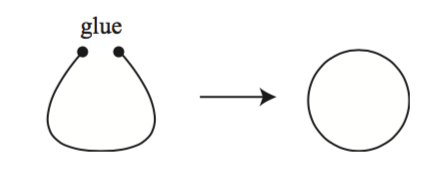
\includegraphics[width=6cm]{week3/p_1}
\caption{Diagram for mapping $f$}
\label{fig:3:1}
\end{figure}
The answer is no, since the left in~(\ref{fig:3:1}) can be isomorphically mapped into $(0,1)$; the right can be isomorphically mapped into $[0,1]$, and the mapping $(0,1)\to[0,1]$ cannot be isomorphism:
\begin{proof}
Assume otherwise the mapping $g:(0,1)\to[0,1]$ is isomorphism, and therefore $f^{-1}(U)$ is open for any open set $U$ in the space $[0,1]$.

Construct $U=(1-\delta,1]$ for $\delta\le1$, and therfore $f^{-1}((1-\delta,1])$ is open, and therfore for the point $x=f^{-1}(1)$, there exists $\varepsilon>0$ such that
\[
B_{\varepsilon}(x)\subseteq f^{-1}((1-\delta,1])
\implies
[x-\varepsilon,x)\subseteq f^{-1}((1-\delta,1)),
\text{ and }
(x,x+\varepsilon]\subseteq f^{-1}((1-\delta,1)).
\]
which implies that there exists $a,b$ such that $[x-\varepsilon,x)=f^{-1}((a,1))$ and $(x,x+\varepsilon]=f^{-1}((b,1))$, i.e., $f^{-1}((a,b)\cap(b,1))$ admits into two values in $[x-\varepsilon,x)$ and $(x,x+\varepsilon]$, which is a contradiction.
\end{proof}
\item
Basis of a topology $\mathcal{B}\subseteq(X,\mathcal{T})$ is a collection of open sets in the space such that the whole space can be recovered, or equivalently
\begin{enumerate}
\item
$\mathcal{B}\subseteq\mathcal{T}$
\item
Every set in $\mathcal{T}$ can expressed as a union of sets in $\mathcal{B}$
\end{enumerate}
Example: Let $\mathbb{R}^n$ be equipped with usual topology, then
\[
B=\{B_q(x)\mid x\in\mathbb{Q}^n,q\in\mathbb{Q}^+\}\ \text{is a basis of $\mathbb{R}^n$. }
\]
It suffices to show $U\subseteq\mathbb{R}^n$ can be written as 
\[
U=U_{x\in\mathbb{Q}}B_{q_x}(x)
\]
\end{enumerate}

\begin{proposition}
Let $X,Y$ be topological spaces, and $\mathcal{B}$ a basis for topology on $Y$. Then
\[
f:X\to Y\text{ is continuous}
\Longleftrightarrow
f^{-1}(B)\text{ is open in X, }\forall B\in\mathcal{B}
\]
Therefore checking $f^{-1}(U)$ is open for all $U\in\mathcal{T}_Y$ suffices to checking $f^{-1}(N)$ is open for all $B\in\mathcal{B}$.
\end{proposition}

\begin{proof}
The forward direction follows from the fact $B\subseteq\mathcal{T}_Y$.

To show the reverse direction, let $U\in\mathcal{T}_Y$, then $U=\bigcup_{i\in I}B_i$, where $B_i\in\mathcal{B}$, which implies
\[
f^{-1}(U)=f^{-1}\left(
\bigcup_{i\in I}B_i
\right)
=
\bigcup_{i\in I}f^{-1}(B_i)
\]
which is open in $X$ by our hypothesis.
\end{proof}

\begin{corollary}\label{cor:3:1}
Let $f:X\to Y$ be a bijection. Suppose there is a basis $\mathcal{B}_X$ of $\mathcal{T}_X$ such that $\{f(B)\mid B\in\mathcal{B}_X\}$ forms a basis of $\mathcal{T}_Y$. Then $X\cong Y$.
\end{corollary}
\begin{proof}
Suppose $W\in\mathcal{T}_Y$, then by our hypothesis,
\[
W=\bigcup_{i\in I}f(B_i),\
B_i\in\mathcal{B}_X\implies
f^{-1}(W)=\bigcup_{i\in I}B_i\in\mathcal{T}_X,
\]
which implies $f$ is continuous.

Suppose $U\in\mathcal{T}_X$, then
\[
U=\bigcup_{i\in I}B_i\implies
f(U)=\bigcup_{i\in I}f(B_i)\in\mathcal{T}_Y\implies
[f^{-1}]^{-1}(U)\in\mathcal{T}_Y,
\]
i.e., $f^{-1}$ is continuous.
\end{proof}

Question: \textit{how to recognise 
whether a family of subsets is a basis for some given topology?}

\begin{proposition}
\label{pro:3:4:1}
Let $X$ be a set, $\mathcal{B}$ is a collection of subsets satisfying
\begin{enumerate}
\item
$X$ is a union of sets in $\mathcal{B}$, i.e., 
every $x\in X$ lies in some $B_x\in\mathcal{B}$
\item
The intersection $B_1\cap B_2$ for $\forall B_1,B_2\in\mathcal{B}$ is a union of sets in $\mathcal{B}$, i.e., for each $B_1,B_2\in\mathcal{B}$, and $x\in B_1\cap B_2$, then there exists $B_3\in\mathcal{B}$ such that $x\in B_3\subseteq B_1\cap B_2$.
\end{enumerate}
Then the collection of subsets $\mathcal{T}_{\mathcal{B}}$, formed by taking any union of sets in $\mathcal{B}$, is a topology, and $\mathcal{B}$ is a basis for $\mathcal{T}_B$.
\end{proposition}

\begin{proof}
\begin{enumerate}
\item
$\emptyset\in\mathcal{T}_{\mathcal{B}}$ (taking nothing from $\mathcal{B}$); for $x\in X,B_x\in\mathcal{B}$, by hypothesis~(1),
\[
X=\bigcup_{x\in X}B_x\in\mathcal{T}_{\mathcal{B}}
\]
\item
Suppose $T_1,T_2\in\mathcal{T}_{\mathcal{B}}$. Let $x\in T_1\cap T_2 $, 
where $T_i$ is a union of subsets in $\mathcal{B}$. Therefore,
\[
\left\{
\begin{aligned}
x\in B_1\subseteq T_1,\qquad B_1\in\mathcal{B}\\
x\in B_2\subseteq T_2,\qquad B_2\in\mathcal{B}
\end{aligned}
\right.
\]
which implies $x\in B_1\cap B_2$, i.e., $x\in B_x\subseteq B_1\cap B_2$ for some $B_x\in\mathcal{B}$.
Therefore,
\[
\bigcup_{x\in B_1\cap B_2}\{x\}\subseteq
\bigcup_{x\in B_1\cap B_2}B_x\subseteq B_1\cap B_2,
\]
i.e., $B_1\cap B_2=\bigcup_{x\in B_1\cap B_2}B_x$, i.e., $B_1\cap B_2\in\mathcal{T}_{\mathcal{B}}$.
\item
The property that $\mathcal{T}_{\mathcal{B}}$ is closed under union operations can be checked directly.
\end{enumerate}
The proof is complete.
\end{proof}

\subsection{Product Space}
Now we discuss how to construct new topological spaces out of given ones is by taking Cartesian products:
\begin{definition}\label{def:3:4}
Let $(X,\mathcal{T}_X),(Y,\mathcal{T}_Y)$ be topological spaces. Consider the family of subsets in $X\times Y$:
\[
\mathcal{B}_{X\times Y}=\{U\times V\mid U\in\mathcal{T}_X,V\in\mathcal{T}_y\}
\]
This $\mathcal{B}_{X\times Y}$ forms a basis of a topology on $X\times Y$. The induced topology from $\mathcal{B}_{X\times Y}$ is called \emph{product topology}.
\end{definition}

For example, for $X=\mathbb{R},Y=\mathbb{R}$, the elements in $\mathcal{B}_{X\times Y}$ are rectangles.
\begin{proof}[Proof for well-definedness in definition~(\ref{def:3:4})]
We apply proposition~(\ref{pro:3:4:1}) to check whether $B_{X\times Y}$ forms a basis:
\begin{enumerate}
\item
For any $(x,y)\in X\times Y$, we imply $x\in X,y\in Y$. Note that $X\in\mathcal{T}_X,Y\in\mathcal{T}_Y$, we imply $(x,y)\in X\times Y\in\mathcal{B}_{X\times Y}$.
\item
Suppose $U_1\times V_1,U_2\times V_2\in\mathcal{B}_{X\times Y}$, then 
\[
(U_1\times V_1)\cap(U_2\times V_2)=(U_1\cap U_2)\times (V_1\cap V_2),
\]
where $U_1\cap U_2\in\mathcal{T}_X,V_1\cap V_2\in\mathcal{T}_Y$. Therefore, $(U_1\times V_1)\cap(U_2\times V_2)\in\mathcal{B}_{X\times Y}$.
\end{enumerate}
\end{proof}
\begin{remark}
However, the product topology may not necessarily become the largest topology in the space $X\times Y$. Consider $X=\mathbb{R},Y=\mathbb{R}$, the open set in the space $X\times Y$ may not necessarily be rectangles. However, all elements in $\mathcal{B}_{X\times Y}$ are rectangles.
\end{remark}




\begin{example}
The space $\mathbb{R}\times\mathbb{R}$ is homeomorphic to $\mathbb{R}^2$, where the product topology is defined on $\mathbb{R}\times\mathbb{R}$ and the standard topology is defined on $\mathbb{R}^2$:

Construct the function $f:\mathbb{R}\times\mathbb{R}\to\mathbb{R}^2$ with $(a,b)\to(a,b)$.

Obviously, $f:\mathbb{R}\times\mathbb{R}\to\mathbb{R}^2$ is a bijection.

Take the basis of the topology on $\mathbb{R}$ as open intervals,
\[
B_X=\{(a,b)\mid a<b\text{ in $\mathbb{R}$}\}
\]
Therefore, one can verify that the set $\mathcal{B}:=\{(a,b)\times(c,d)\mid a<b,c<d\}$ forms a basis for the product topology, and 
\[
\{f(B)\mid B\in\mathcal{B}\}=\{(a,b)\times(c,d)\mid a<b,c<d\}
\]
forms a basis of the usual topology in $\mathbb{R}^2$.

By Corollary~(\ref{cor:3:1}), we imply $\mathbb{R}\times\mathbb{R}\cong\mathbb{R}^2$.
\end{example}
We also raise an example on the homeomorphism related to product spaces:
\begin{example}
Let $S^1=\{(\cos x,\sin x\mid x\in[0,2\pi])\}$ be a unit circle on $\mathbb{R}^2$.

Consider $f: S^1\times(0,\infty)\to\mathbb{R}^2\setminus\{\bm0\}$ defined as
\[
f(\cos x,\sin x,r)\mapsto(r\cos x,r\sin x)
\]
It's clear that $f$ is a bijection, and $f$ is continuous. 
Moreover, the inverse $g:=f^{-1}$ is defined as
\[
g(a,b)=(\frac{a}{\sqrt{a^2+b^2}},\frac{b}{\sqrt{a^2+b^2}},\sqrt{a^2+b^2})
\]
which is continuous as well.
Therefore, the $f:\mathcal{S}^1\times(0,\infty)\to\mathbb{R}^2\setminus\{\bm0\}$ is a homeomorphism.
\end{example}
















